\documentclass[tikz,border=8pt]{standalone}
\usetikzlibrary{arrows.meta,positioning,shapes.misc}

\definecolor{spaceblue}{RGB}{32,105,180}
\definecolor{slopegreen}{RGB}{32,145,105}

\begin{document}
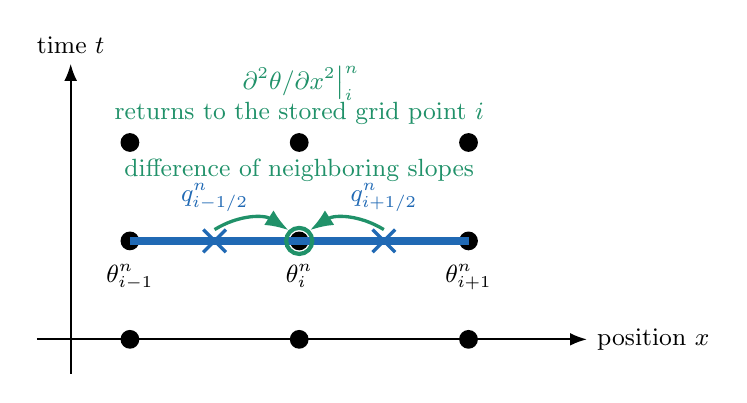
\begin{tikzpicture}[
    x=2.15cm,
    y=1.25cm,
    >=Latex,
    node/.style={circle,fill=black,inner sep=2.4pt},
    midpoint/.style={cross out,draw,line width=1.2pt,minimum size=7pt},
    every node/.style={font=\small}
]
  \draw[->,line width=0.7pt] (-1.55,0) -- (1.70,0) node[right] {position $x$};
  \draw[->,line width=0.7pt] (-1.35,-0.35) -- (-1.35,2.80) node[above] {time $t$};

  \foreach \i in {-1,0,1}
    \foreach \n in {0,1,2}
      \node[node] at (\i,\n) {};

  \draw[spaceblue,line width=2.6pt] (-1,1) -- (0,1);
  \draw[spaceblue,line width=2.6pt] (0,1) -- (1,1);
  \node[midpoint,spaceblue] (leftslope) at (-0.5,1) {};
  \node[midpoint,spaceblue] (rightslope) at (0.5,1) {};
  \node[below=5pt] at (-1,1) {$\theta_{i-1}^n$};
  \node[below=5pt] at (0,1) {$\theta_i^n$};
  \node[below=5pt] at (1,1) {$\theta_{i+1}^n$};
  \node[spaceblue,above=7pt] at (-0.5,1) {$q_{i-1/2}^n$};
  \node[spaceblue,above=7pt] at (0.5,1) {$q_{i+1/2}^n$};

  \node[draw=slopegreen,circle,line width=1.5pt,minimum size=8pt] (center) at (0,1) {};
  \draw[slopegreen,->,line width=1.2pt,bend left=32]
    (leftslope.north) to (center.north west);
  \draw[slopegreen,->,line width=1.2pt,bend right=32]
    (rightslope.north) to (center.north east);
  \node[slopegreen] at (0,1.72) {difference of neighboring slopes};
  \node[slopegreen,align=center,text width=5.4cm] at (0,2.48)
    {$\left.\partial^2\theta/\partial x^2\right|_i^n$\\returns to the stored grid point $i$};
\end{tikzpicture}
\end{document}
